\section{单形}
\sourcepage{2--3}
在定义单纯同调群之前，必须先讨论它们所适用的空间类，即所有多面体构成的空间类。\textbf{多面体}（polyhedron）是以线段、三角形、四面体及其高维类似物为基本构件，沿着这些构件的面粘合而成的空间。本节讨论这些基本构件；下一节将用它们构造多面体。

首先，需要研究一点欧氏空间的解析几何。用 $\R^N$ 表示 $N$ 维欧氏空间，以 $0$ 表示欧氏空间的原点。对于 $x=(x_1,x_2,\ldots,x_N)\in\R^N$，$x$ 的\textbf{范数}定义为
\[
\|x\|=\left[\sum_{i=1}^N(x_i)^2\right]^{1/2}.
\]
给定 $\R^N$ 中的点集 $\{a_0,a_1,\ldots,a_n\}$，如果对任意实数 $t_i$，等式
\[
\sum_{i=0}^n t_i=0,\qquad \sum_{i=0}^n t_i a_i=0
\]
都蕴含 $t_0=t_1=\cdots=t_n=0$，就称这个点集是\textbf{几何独立的}（geometrically independent）。

显然，单点集总是几何独立的。简单的代数运算表明，一般地，$\{a_0,a_1,\ldots,a_n\}$ 几何独立，当且仅当向量
\[
a_1-a_0,\ a_2-a_0,\ \ldots,\ a_n-a_0
\]
在线性代数的意义下线性无关。因此，$\R^N$ 中两个不同的点构成几何独立集；三个不共线的点、四个不共面的点等也同样如此。

给定几何独立点集 $\{a_0,a_1,\ldots,a_n\}$，定义这些点\textbf{张成的 $n$ 维平面} $P$ 为满足下式的所有点 $x\in\R^N$ 构成的集合：存在标量 $t_i$，使得
\[
x=\sum_{i=0}^n t_i a_i,\qquad \sum_{i=0}^n t_i=1.
\]
由于各 $a_i$ 几何独立，各 $t_i$ 由 $x$ 唯一确定。注意，每个点 $a_i$ 本身都属于平面 $P$。

平面 $P$ 也可描述为所有满足下式的点 $x$ 构成的集合：存在标量 $t_1,\ldots,t_n$，使得
\[
x=a_0+\sum_{i=1}^n t_i(a_i-a_0).
\]
采用这种形式时，我们称 $P$ 为“过 $a_0$ 且平行于向量 $a_i-a_0$ 的平面”。

容易验证，如果 $\{a_0,a_1,\ldots,a_n\}$ 几何独立，并且 $w$ 位于这些点张成的平面之外，那么 $\{w,a_0,a_1,\ldots,a_n\}$ 几何独立。

$\R^N$ 的\textbf{仿射变换}（affine transformation）$T$ 是由平移与非奇异线性变换复合而成的映射；这里，平移是指对某个固定的 $p$，具有形式 $T(x)=x+p$ 的映射。从定义立即可知，仿射变换保持点集的几何独立性，而且把 $\{a_0,\ldots,a_n\}$ 张成的平面 $P$ 映到 $\{T(a_0),\ldots,T(a_n)\}$ 张成的平面上。

现在，平移 $T(x)=x-a_0$ 把 $P$ 映到 $\R^N$ 中以 $a_1-a_0,\ldots,a_n-a_0$ 为基的向量子空间上。在 $T$ 之后，再复合一个把这些向量映为 $\R^N$ 中前 $n$ 个单位基向量 $\epsilon_1,\ldots,\epsilon_n$ 的线性变换，就得到 $\R^N$ 的一个仿射变换 $S$，使得 $S(a_0)=0$，并且当 $i>0$ 时，$S(a_i)=\epsilon_i$。\translatornote{原文此处写作 $S(s_0)=0$，其中 $s_0$ 未定义；据上下文应为 $a_0$。}映射 $S$ 把 $P$ 映到 $\R^N$ 中由前 $n$ 个坐标确定的平面 $\R^n\times0$ 上。由此便清楚，为什么称 $P$ 为 $\R^N$ 中的“$n$ 维平面”。

\sourcepage{4}
\entry{定义}{1.2.1}设 $\{a_0,a_1,\ldots,a_n\}$ 是 $\R^N$ 中的几何独立集。定义由 $a_0,a_1,\ldots,a_n$ 张成的 \textbf{$n$ 维单形}（$n$-simplex）$\sigma$ 为满足下式的所有点 $x\in\R^N$ 构成的集合：
\[
x=\sum_{i=0}^n t_i a_i,\qquad
\sum_{i=0}^n t_i=1,\quad t_i\geq0\ \text{对所有 }i.\tag{$*$}
\]
各数 $t_i$ 由 $x$ 和条件 $(*)$ 唯一确定，称为点 $x$ 关于 $a_0,a_1,\ldots,a_n$ 的\textbf{重心坐标}（barycentric coordinates）。

\entry{例}{1.2.2}在低维情形，很容易画出单形。当然，$0$ 维单形就是一个点。由 $a_0$ 和 $a_1$ 张成的 $1$ 维单形由所有形如
\[
x=ta_0+(1-t)a_1,\qquad 0\leq t\leq1
\]
的点组成，因此就是连接 $a_0$ 与 $a_1$ 的线段。这个线段可记作 $a_0a_1$。

类似地，由 $a_0,a_1,a_2$ 张成的 $2$ 维单形 $\sigma$ 就是以这三个点为顶点的三角形区域。最容易看出这一点的方法如下。设 $x\ne a_0$，则
\[
x=\sum_{i=0}^2t_i a_i
=t_0a_0+(1-t_0)\bigl[(t_1/\lambda)a_1+(t_2/\lambda)a_2\bigr],
\]
其中 $\lambda=1-t_0$。方括号中的表达式表示连接 $a_1$ 与 $a_2$ 的线段上的一个点 $p$，因为 $(t_1+t_2)/\lambda=1$，且对 $i=1,2$ 有 $t_i/\lambda\geq0$。因此，$x$ 是连接 $a_0$ 与 $p$ 的线段上的一个点，见图 1.2.1。

反过来，可以验证，这样的线段上的每个点都属于 $\sigma$。因此，$\sigma$ 等于连接 $a_0$ 与 $a_1a_2$ 上各点的所有线段的并。也就是说，$\sigma$ 是一个三角形区域，可以记作 $a_0a_1a_2$。
\begin{center}
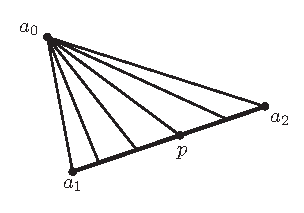
\includegraphics[width=50mm]{figures/1-2-1.pdf}\\图 1.2.1
\end{center}
类似的证明表明，$3$ 维单形就是四面体。

\sourcepage{5}
\entry{定义}{1.2.3}
\begin{enumerate}[label=(\alph*)]
\item 设 $\sigma$ 是由几何独立的点 $a_0,a_1,\ldots,a_n$ 张成的单形。各点 $a_i$ 称为 $\sigma$ 的\textbf{顶点}（vertex），数 $n$ 称为 $\sigma$ 的\textbf{维数}（dimension）。可以把 $\sigma$ 记作 $a_0a_1\cdots a_n$。
\item 由 $\{a_0,a_1,\ldots,a_n\}$ 的某个子集张成的任何单形，称为 $\sigma$ 的一个\textbf{面}（face）。
\item 设 $s$ 是由 $a_0,a_1,\ldots,a_p$ 张成的面，其中 $p<n$；设 $t$ 是由 $a_{p+1},a_{p+2},\ldots,a_n$ 张成的面。称 $t$ 为 $\sigma$ 中与 $s$ \textbf{相对的面}。特别地，由 $a_1,a_2,\ldots,a_n$ 张成的面称为与 $a_0$ 相对的面。
\item $\sigma$ 的不同于其自身的面称为 $\sigma$ 的\textbf{真面}（proper face）。
\item $\sigma$ 的所有真面的并称为 $\sigma$ 的\textbf{边界}（boundary），记作 $\Bd\sigma$。
\item $\sigma$ 的\textbf{内部}（interior）记作 $\Int\sigma$，定义为 $\Int\sigma=\sigma\setminus\Bd\sigma$。务必注意，$0$ 维单形的内部就是该 $0$ 维单形自身；这可能与你的直觉不同。
\item 集合 $\Int\sigma$ 有时称为\textbf{开单形}（open simplex）。
\end{enumerate}
回顾一些标准记号。\textbf{单位 $n$ 维球} $B^n$ 是 $\R^n$ 中满足 $\|x\|\leq1$ 的所有点 $x$ 构成的集合；\textbf{单位球面} $S^{n-1}$ 是满足 $\|x\|=1$ 的点集。$S^{n-1}$ 的\textbf{上半球面} $E_+^{n-1}$ 由其中满足 $x_n\geq0$ 的点组成；\textbf{下半球面} $E_-^{n-1}$ 由其中满足 $x_n\leq0$ 的点组成。

依照这些定义，$B^0$ 是单点空间，$B^1$ 等于区间 $[-1,1]$，$S^0$ 是两点空间 $\{-1,1\}$。二维球是 $\R^2$ 中以原点为中心的单位圆盘，而 $S^1$ 是单位圆周。

\entry{定义}{1.2.4}若对于 $\R^N$ 的子集 $A$ 中任意两点 $x,y$，连接它们的线段都包含在 $A$ 中，则称 $A$ 是\textbf{凸的}（convex）。

还有一个较弱的定义，有时也很有用。

\entry{定义}{1.2.5}若对于 $A\subset\R^N$ 中每个不同于 $w\in A$ 的点 $x$，连接 $x$ 与 $w$ 的线段都包含在 $A$ 中，则称 $A$ \textbf{关于点 $w$ 星形凸}（star-convex）。

下面列出单形的一些基本性质。证明都是初等的，大部分留作习题。

\entry{引理}{1.2.6}设 $P$ 是由几何独立集 $\{a_0,a_1,\ldots,a_n\}$ 确定的 $n$ 维平面，$\sigma$ 是由这些点张成的 $n$ 维单形。
\begin{enumerate}[label=(\arabic*)]
\item 点 $x$ 关于 $a_0,a_1,\ldots,a_n$ 的重心坐标 $t_i(x)$ 是 $x$ 的连续函数。
\item 单形 $\sigma$ 等于连接 $a_0$ 与单形 $s=a_1\cdots a_n$ 中各点的所有线段的并。这样的两条不同线段仅在 $a_0$ 处相交。
\item 单形 $\sigma$ 是 $\R^N$ 中的紧致凸集，并且等于 $\R^N$ 中所有包含 $a_0,a_1,\ldots,a_n$ 的凸集的交。
\item 给定单形 $\sigma$，恰好存在一个张成 $\sigma$ 的几何独立点集。
\item 集合 $\Int\sigma$ 是凸的，在平面 $P$ 中是开集，其闭包为 $\sigma$。此外，$\Int\sigma$ 等于连接 $a_0$ 与 $\Int s$ 中各点的所有开线段的并，其中 $s$ 是 $\sigma$ 中与 $a_0$ 相对的面。
\item 存在从 $\sigma$ 到单位球 $B^n$ 的同胚，它把 $\Bd\sigma$ 映到单位球面 $S^{n-1}$ 上。
\end{enumerate}
\noindent\textbf{证明：}第 (1)--(5) 项留作习题。第 (6) 项是下一个引理的推论；后者是一个更强的结果，在后文也有用。

\sourcepage{6--7}
对于拓扑空间的子集 $A$，我们用 $\overline A$ 表示其闭包，用 $\Int A$ 表示其内部，用 $\Bd A=\overline A\setminus\Int A$ 表示其边界。

\entry{引理}{1.2.7}设 $U$ 是 $\R^n$ 中的有界凸开集，$w\in U$。
\begin{enumerate}[label=(\alph*)]
\item 从 $w$ 出发的每条射线与 $\Bd U=\overline U\setminus U$ 恰好相交于一点。
\item 存在从 $\overline U$ 到 $B^n$ 的同胚，它把 $\Bd U$ 映到 $S^{n-1}$ 上。
\end{enumerate}
\noindent\textbf{证明：}
(a) 给定一条从 $w$ 出发的射线 $R$，其与 $U$ 的交是凸的、有界的，并且在 $R$ 中是开集。因此，这个交由所有形如 $w+tp$ 的点组成，其中 $t$ 遍历某个半开区间 $[0,a)$。所以，点 $x=w+ap$ 是 $R$ 上属于 $\overline U\setminus U$ 的一个点。

假设 $R$ 与 $\overline U\setminus U$ 还相交于另一点 $y$，则对于某个 $b>a$，有 $y=w+bp$。可以写成
\[
x=(1-t)w+ty,\qquad t=a/b.
\]
将其改写为
\[
w=(x-ty)/(1-t).
\]
取 $U$ 中的点列 $y_n$ 收敛于 $y$，并定义
\[
w_n=(x-ty_n)/(1-t).
\]
见图 1.2.2。点列 $w_n$ 收敛于 $w\in U$，所以当某个 $n$ 足够大时，$w_n\in U$。于是，由于 $x=tw_n+(1-t)y_n$，且 $U$ 是凸集，便有 $x\in U$，与 $x$ 的选取矛盾。\translatornote{原文等式为 $x=tw_n+(1-t)y_n$；由上文 $w_n$ 的定义，应为 $x=(1-t)w_n+ty_n$。两系数均在 $(0,1)$ 内，使用正确等式即得所需矛盾。}
\begin{center}
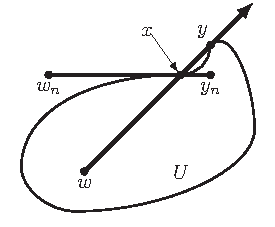
\includegraphics[width=48mm]{figures/1-2-2.pdf}\\图 1.2.2
\end{center}
(b) 为方便起见，设 $w=0$。等式 $f(x)=x/\|x\|$ 定义了从 $\R^n\setminus\{0\}$ 到 $S^{n-1}$ 的连续满射 $f$。由 (a)，$f$ 在 $\Bd U$ 上的限制是到 $S^{n-1}$ 的双射。由于 $\Bd U$ 紧致，这个限制映射是同胚，记其逆映射为 $g$。将 $g$ 扩张成双射 $G:B^n\to\overline U$，使 $G$ 把连接 $0$ 与 $u\in S^{n-1}$ 的线段线性地映到连接 $0$ 与 $g(u)$ 的线段上。具体地，定义
\[
G(x)=\begin{cases}
\|g(x/\|x\|)\|x,&x\ne0,\\
0,&x=0.
\end{cases}
\]
当 $x\ne0$ 时，$G$ 的连续性是显然的。在 $0$ 处的连续性也很容易证明：若 $M$ 是 $\|g(x)\|$ 的一个上界，那么只要 $\|x-0\|<\delta$，就有 $\|G(x)-G(0)\|<M\delta$。\hfill$\square$

\subsection*{习题}
\begin{enumerate}
\item 验证引理 1.2.6 的第 (1)--(3) 项。［提示：若 $T$ 是将 $a_0$ 映为 $0$、将 $a_i$ 映为 $\epsilon_i$ 的仿射变换，那么 $T$ 将点 $x=\sum_{i=0}^n t_i a_i$ 映为点 $(t_1,t_2,\ldots,t_n,0,\ldots,0)$。］
\item 按下列步骤验证引理 1.2.6 的第 (4) 项：
\begin{enumerate}[label=(\alph*)]
\item 证明：如果 $x\in\sigma$ 且 $x\ne a_0,a_1,\ldots,a_n$，那么 $x$ 位于某条包含在 $\sigma$ 中的开线段上。［设 $n>0$。］
\item 证明 $a_0$ 不位于任何包含在 $\sigma$ 中的开线段上。为此证明：若 $a_0=tx+(1-t)y$，其中 $x,y\in\sigma$ 且 $0<t<1$，则 $x=y=a_0$。
\end{enumerate}
\item 验证引理 1.2.6 的第 (5) 项。
\item 如下推广引理 1.2.6 的第 (2) 项。设 $\sigma$ 由 $a_0,a_1,\ldots,a_n$ 张成，$s$ 是由 $a_0,a_1,\ldots,a_p$ 张成的面，其中 $p<n$，而 $t$ 是与 $s$ 相对的面。
\begin{enumerate}[label=(\alph*)]
\item 证明 $\sigma$ 是连接 $s$ 中各点与 $t$ 中各点的所有线段的并，且其中任意两条不同线段至多相交于一个公共端点。
\item 证明 $\Int\sigma$ 是连接 $\Int s$ 中各点与 $\Int t$ 中各点的所有开线段的并。
\end{enumerate}
\item 设 $U$ 是 $\R^n$ 中的有界开集，且 $U$ 关于原点星形凸。
\begin{enumerate}[label=(\alph*)]
\item 证明，从 $0$ 出发的一条射线可能与 $\Bd U$ 相交于多于一个点。
\item[\textasteriskcentered\,(b)] 举例说明，$U$ 不一定与 $B^n$ 同胚。
\end{enumerate}
\end{enumerate}
